\chapter{Parte I}

\section{Generazione delle copie}
L'obiettivo è quello di generare delle copie non troppo differenti dagli originali. Abbiamo provato varie tecniche, tra le quali:
\begin{itemize}
	\item aggiungere un unico valore randomico a tutti i campioni dello spettro
	\item moltiplicare tutti i campioni per un valore randomico
	\item dividere lo spettro in tre parti uguali e, per ognuno, aggiungere un valore randomico costante
	\item lo stesso del punto precedente, ma moltiplicando invece che addizionando il valore
\end{itemize}

Tutti i metodi sono risultati efficaci con una buona regolazione del range di generazione dei valori randomici. L'addizione e la moltiplicazione sono sostanzialmente equivalenti, anche se i coefficienti hanno un diverso peso sul rumore. Per questioni di comodità abbiamo scelto il metodo moltiplicativo. Resta da decidere se utilizzare un unico valore moltiplicativo su tutto lo spettro oppure dividere lo spettro in tre parti uguali sulla quale aggiungere il rumore. Abbiamo scelto di fare entrambe le cose per generalizzare la funzione di fitting della rete neurale.

Per ogni colore del set master generiamo 10 copie, di cui 5 sono disturbate costantemente e le restanti 5 sono disturbate su 3 fasce diverse dello spettro. Forniamo alcuni esempi significativi di coppie di colore generate (originale, copia).

\begin{figure}
\begin{center}
	
\includegraphics[scale=0.5]{images/rete1-colore1.PNG}
	
\includegraphics[scale=0.5]{images/rete1-colore2.PNG}
	
\includegraphics[scale=0.5]{images/rete1-colore3.PNG}
	
\includegraphics[scale=0.5]{images/rete1-colore4.PNG}
\end{center}
\caption{Esempi di copie generate (originale, copia)}
\end{figure}

Dopo una verifica visiva possiamo monitorare di quanto le copie siano state disturbate, in modo aggregato, rispetto al colore master. Il metodo suggerito dalle specifiche è quello della distanza euclidea (\(de()\) per MATLab), che calcoliamo per ogni coppia (master, copia). Possiamo ora usare il vettore delle distanze come input per un istogramma.

\begin{figure}
\begin{center}
	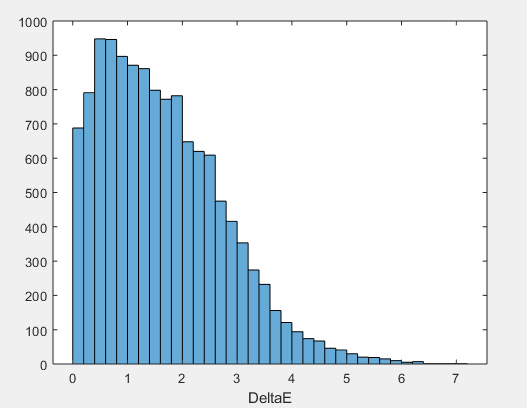
\includegraphics[scale=0.8]{images/rete1-istogramma-deltae.PNG}
\end{center}
\caption{Istogramma delle DeltaE delle coppie (master, copia disturbata)}
\end{figure}

Dal grafico è possibile notare come le coppie stiano nel range 0-4 circa, confermando il fatto che le copie generate siano più o meno simili a quelle originali, come richiesto dalle specifiche.

\section{Features}
A questo punto dobbiamo scegliere quale feature estrarre. Abbiamo ragionato principalmente sul materiale fornito dalle specifiche, in particolare su come viene calcolato il colore percepito dall'occhio umano secondo gli standard CIE. Abbiamo preso in considerazione diverse funzioni, cioè \textit{mean, mode, median, sum, skewness, kurtosis, min and max (sia massimi/minimi che punti di massimo/minimo)}. Ognuna di queste è applicata su 3 range diversi dello spettro (3 range della stessa dimensione), quindi ogni funzione produce tre feature.

Il metodo utilizzato per la feature extraction è quello fornito da MATLab attraverso la funzione \textit{sequentialfs()}. Il numero di feature estratte è stato oggetto di analisi al fine di individuare il minor numero di feature (ne vogliamo meno possibili per semplificare la rete) e ottenere le migliori prestazioni della rete neurale.

SEEDSET

\section{Risultati}
Abbiamo riscontrato un problema nel dataset fornito, in particolare per quanto riguarda le coordinate \textit{Lab}: provando a ricalcolarle partendo dagli spettri di (\textit{spectra}) sono state notate delle differenze nei valori, anche se non sostanziali (un errore di circa \(+- 0.1\)). Per questo motivo abbiamo scelto di usare le coordinate calcolate usando la \textit{roo2lab()} invece di quelle già fornite.

La rete che ha i risultati migliori è quella con 12 neuroni nello strato di ingresso e 10 nell'hidden layer (unico strato): il risultato è quantificabile in Mean Squared Error pari a circa 0.017 e un valore R (regressione) pari a 0.99338.

\begin{figure}
\begin{center}
	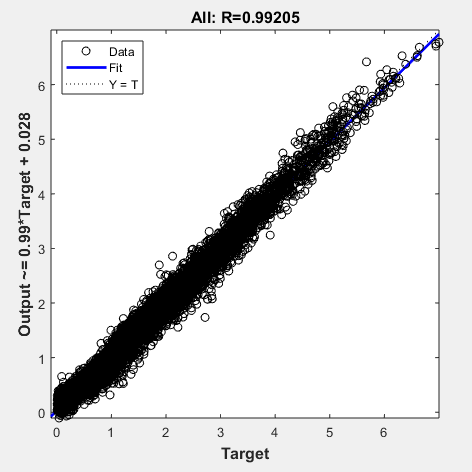
\includegraphics[scale=0.7]{images/rete1-regression.jpg}
\end{center}
\caption{Retta di Regressione della rete neurale}
\end{figure}

\paragraph{Feature estratte}
Le feature estratte dalla \textit{sequentialfs} sono state le seguenti:
\\\\
\textbf{master}: mean(2), mode(3), median(4), median(5), skewness(3), maxYValue(2), minYValue(1)
\\
\textbf{copie}: mean(2), var(2), mode(1), skewness(3), maxYValue(2)
\\\\(1,2,3) indicano i 3 range dello spettro equidimensionati sulla quale le funzioni sono applicate
\\(4,5) sono 2 range aggiuntivi, che si sovrappongono ai precedenti (dividono lo spettro in 2)

Tuttavia differenti esecuzioni hanno portato, spesso, all'estrazione di feature differenti: questo può essere dovuto alla correlazione tra le varie funzioni scelte (es. la skewness è calcolata dal mean e dalla varianza).